
\documentclass[12pt]{article}

\title{The Public Factor Exposure of Private Equity}

\author{
	Christian Tausch  \\
	AssetMetrix GmbH  \\
	Theresienh\"{o}he 13, D-80339 Munich \\
	christian.tausch@quant-unit.com \\
	\and 
	Marcus Pietz  \\
	AssetMetrix GmbH  \\
	Theresienh\"{o}he 13, D-80339 Munich \\
	marcus.pietz@asset-metrix.com \\
	}

\date{\today}



% Packages
\usepackage{amssymb}
\usepackage{amsmath}
\usepackage{natbib}
\usepackage{graphics}
% use smaller margins
\usepackage[margin=1.1in]{geometry} % 1.25in
\usepackage[margin=1.1cm]{caption}
% use double spacing
\usepackage{setspace}
\usepackage{amsthm}
\usepackage{url}
\usepackage[outdir=./]{epstopdf}
\usepackage{booktabs}
\usepackage{float}
\usepackage{standalone}


\newtheorem{prop}{Proposition}
\newtheorem{assume}{Assumption}


% logo
\usepackage{fancyhdr}
\usepackage{graphicx }

\iffalse
%\addtolength{\headheight}{1cm} % make more space for the header
\pagestyle{fancyplain} % use fancy for all pages except chapter start
\lhead{
\includegraphics[height=0.6cm]{logo/quantunitcom}} % left logo
\rhead{
\includegraphics[height=0.6cm]{logo/AssetMetrixLogo2019schwarz}} % right logo
%\renewcommand{\headrulewidth}{0pt} % remove rule below header
\renewcommand{\chaptermark}[1]{ \markboth{#1}{} }
\renewcommand{\sectionmark}[1]{ \markright{#1}{} }
\fi


\begin{document}

\maketitle


\section*{Keywords}
 Public factor exposure, Private equity, Stochastic discount factor, Model combination, Factor investing, Ensemble learning


\section*{Acknowledgements}
We thank Nicolas D\"{u}tsch and Philipp Abel for valuable feedback and helpful comments that greatly improved the paper.


\section*{Declaration of interest}
The authors report no conflict of interest. 
The authors alone are responsible for the content and writing of the paper.


\newpage
%\doublespacing

\begin{center} 
\section*{The Public Factor Exposure of Private Equity}
\end{center}


\abstract{
	We propose Stochastic Discount Factor (SDF) model combination to determine the public factor exposure of private equity.
	First, we describe our theoretical motivation to favor model combination over model selection.
	This entails that we apply simple coefficient averaging to obtain multivariate SDF models that mimic the factor exposure of all major private capital fund types.
	As a next step, we suggest componentwise $L_2$ boosting to estimate the error term time series associated with our factor models.
	The empirical results indicate that the replication strategies for the most conventional private equity fund types slightly outperform the (unlevered) MSCI World index in our sample period.
	Finally, we outline how to employ these factor models for integrated public and private risk management. 
}


\section{Introduction}
\label{sec:factor_investing}

Factor investing is currently popular in public markets as it helps investors to identify underlying return drivers.
Describing a portfolio's public factor exposure corresponds to understanding both its (i) realized returns and (ii) forward-looking risk and return expectations.
Realistic factor decompositions offer nuanced insights also for private market investors, assuming there exist common components that drive public and private returns.
From this viewpoint, factor analysis translates private equity returns to traded return components with main applications in public market equivalent benchmarking and holistic risk management.

Generally, more sophisticated methods are required to estimate factor models for private (in comparison to public) asset classes as private returns are not directly observable on liquid secondary markets.
However, the challenge of identifying the 'best' factor model is the same as in public markets.
There are first attempts to select or create public indices that shall replicate private equity (PE) returns.
Here, we can distinguish between (i) factor- and (ii) holding-based approaches.
\cite{P14} benchmarks buyout funds against several factor indices.
More subtle factor-based methods are mainly established in the hedge fund replication literature \citep{TV08,W14}.
To avoid overfitting, \cite{OST17} propose to combine multiple factor models for passive hedge fund replication.
Holding-based approaches to mimic the PE investment style are proposed by \cite{LSSL16}, \cite{S17}, \cite{MS19}, and \cite{PP19}.
This paper pursues a factor-based solution that employs publicly traded indices and does not require deal-level information on PE funds.
In contrast to the factor-based ansatz of \cite{P14}, we base our approach on SDF models that are actually estimated on PE fund-level data rather than comparing several ad-hoc choices for potentially suitable indices.

This article aims at a data-science-driven solution to describe PE returns\footnote{See \cite{CG23} for a textbook treatment of machine learning methods for factor investing.}.
Concretely, we propose SDF model combination as a straightforward method to obtain 'strong' public factor models that explain private equity returns.
Here, we provisionally define the term 'strong' versus 'weak' model in analogy to the boosting literature \citep{S90}.
A 'strong' model shall exhibit small (error term) bias and variance, whereas a 'weak' model displays high bias and variance.
Only the 'true' or 'best' or 'optimal' model obtains an error term of precisely zero.
Figure \ref{fig:how} illustrates our general ensemble-based approach to derive the public factor exposure of private equity \citep{B12}.

The paper is structured as follows.
Section \ref{sec:semiparametric_setting} introduces the method's underlying semiparametric setting.
Section \ref{sec:model_selection} explains why model selection is problematic.
Section \ref{sec:model_combination} argues that model combination is more promising.
Section \ref{sec:applications} presents two examples of how to apply our combined SDF models in the benchmarking and risk context.
Section \ref{sec:conclusion} concludes.

\begin{figure}[ht]
	\centering
	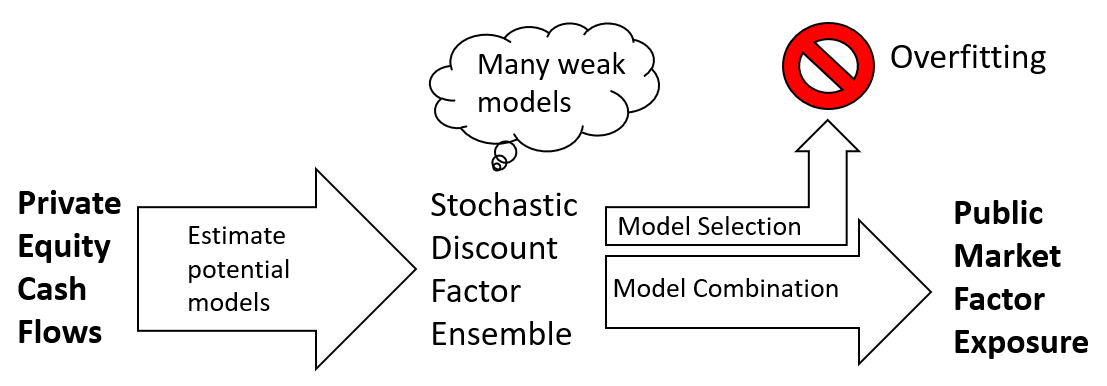
\includegraphics[width=14cm]{FlowChart/FC4}
	\caption{How to translate private equity cash flows to public market factors?}
	\label{fig:how}
\end{figure}

\section{Semiparametric setting}
\label{sec:semiparametric_setting}

Stochastic Discount Factors (SDFs) are econometric models to price a given cash flow stream \citep{HR87}.
They are usually estimated by semiparametric approaches that go without a parametric model for the error term \citep{F19}.
Following \cite{DLP12}, the cash flows stream under consideration is generated by $i=1,2,\dots,n$ private equity funds (or portfolios).
SDFs can be applied in net present value calculations for realized cash flow paths
\begin{equation}
\label{eq:pricing_error}
P_{\tau, i} =
\sum_{t=1}^{T}\ \Psi_{\tau, t}\ {CF}_{t, i}
\end{equation}
with price $P$, SDF functional $\Psi$, and cash flow stream $CF$. 
Time is discrete with $t=1,2,\dots,T$.
If the 'true' SDF model is applied, the expected price\footnote{We also refer to $P$ as pricing error since we want to avoid any average price deviation from zero, i.e., minimize the expected pricing error.} $\mathbb{E}[P]=0$. 
Thus the functional form and explanatory variables used in the 'true' SDF explain or describe the risk and return properties of the cash flows. 
Further, if we have an appropriate SDF for a given private equity fund type, we can apply it in a simple net present value calculation (as in the formula above) to assess the outperformance of a specific private equity fund. 
A positive/negative net present value indicates an out/under-performance compared to other PE funds.
To discount a time $t$ cash flow to time $\tau$, we use the simple linear multi-period SDF model
\begin{equation}
\label{eq:linear_sdf}
\Psi_{\tau,t} =
\frac{
	\prod_{h=0}^{\tau}\ \left(1 + \alpha + r_{h} + \sum_j\ \beta_j\ F_{j,h} + e_h \right)
}{
	\prod_{h=0}^{t}\ \left(1+ \alpha + r_{h} + \sum_j\ \beta_j\ F_{j,h} + e_h \right)
}
\end{equation}
with usually $\alpha=0$, $e_h=0 \ \forall \ h$, risk-free rate $r$, zero-net-investment factor return $F$, and factor coefficient $\beta$ that has to be estimated from data. 
Consequently, the expected multi-period return for a given asset is modeled by
\[
E \left[R_{\tau,t} \right] = 
E \left[ \frac{1}{\Psi_{\tau,t}} + \epsilon_{\tau,t} \right]
\]
where the period-specific error term $\epsilon_{\tau,t}$ has zero expectation $E[\epsilon_{\tau,t}]=0$.

As commonly seen in the asset pricing literature, we estimate SDF model coefficients by semiparametric approaches that require no distributional assumption for $\epsilon_{\tau,t}$.
This means we select $\alpha$ and $\beta$ values that yield average pricing errors close to zero. 
Here the typical loss function choices are quadratic forms like in Generalized Method of Moments (GMM) or a quadratic or least absolute deviance loss function $L()$
\begin{equation}
\label{eq:elastic_net}
\hat{\theta } = \
\arg \min_{\theta} \frac{1}{n} \sum_{i=1}^n L \left( P ; \theta, \gamma \right)
\end{equation}
where $\theta=(\alpha,\beta)$ and $\gamma$ denotes the vector of potential hyperparameters like data cutoff dates or weighting/averaging methods.
More details on the semiparametric estimation framework can be found in the original paper of \cite{DLP12} and its credit market factor application by \cite{HSS23}.
As a little modification of their native method, we average over multiple compounding dates $\tau \in \mathcal{T}$ in our quadratic loss function
\begin{equation}
	\label{eq:quadratic_loss}
	L \left( P ; \theta, \gamma \right) = \left( \frac{1}{|\mathcal{T}|} \sum_{\tau \in \mathcal{T}} P_{\tau,i}  \right)^2
\end{equation}
to decrease the small-sample bias and variance of the estimator.


\section{So many weak SDF model candidates}
\label{sec:model_selection}

In the semiparametric setting described in section \ref{sec:semiparametric_setting}, we likely obtain many weak model candidates with no clear winner among them.
This scenario is comparable to the extensive ``factor model zoo'' observed in public equity markets, as coined by \cite{C11,FGX20}. Furthermore, the extensive body of public market literature fails to definitively determine which factors provide the most comprehensive explanation for their assets' returns.
In this section, we explain in greater detail why we also expect to be confronted with (i) many but (ii) weak SDF model candidates in the private equity case.
Moreover, we discuss why it is challenging to select the single 'best' model from an extensive collection of homogeneous competitors (that all use the same SDF model as specified in equation \ref{eq:linear_sdf}).

\paragraph{Why are there so many models?}

\begin{itemize}
	\item There exists a great variety of different public return factor candidates that might be also relevant for private equity. It is not even clear which factors 'best' explain public equity returns, cf. references in \cite{KN20}. 
	\item We can choose from many feasible semiparametric estimators, loss functions, or ancillary machine learning methods, cf. \cite{GKX20} for a public market overview.
	Additionally, there are discretionary choices for regularization- or other hyper-parameters.
	Further, bootstrapping and other resampling-based techniques may be helpful but likewise dramatically increase the number of model candidates.
	\item In contrast to common public databases available for public equity, the private equity literature has to draw on various private -- often proprietary -- data sources. When estimating the same model on different datasets, the coefficient estimates will differ. Unclear data cutoff dates or horizons exacerbate this issue.
\end{itemize}

\paragraph{Why are the models so weak?}

\begin{itemize}
	\item Private equity data is notoriously sparse as the first PE funds were established in the 1970s to 80s. Moreover, it is currently (almost) impossible to collect data on all funds from a given vintage. These issues render finite [infinite] sample inference more [less] reliable.
	\item For fund-level data, the dependency issue introduced by overlapping fund cash flows further reduces the number of independent observations. Similarly, financial engineering applied on fund level like bridge financing or NAV facilities undermine the explanatory power of observed fund cash flows.
	\item In private equity, limited sample sizes typically allow the inclusion of just 1-2 factors in a SDF model; even many two-factor models appear to be statistically insignificant (weak models); models with more covariates almost surely overfit (invalid models).
\end{itemize}

\paragraph{Why is model selection difficult?}

\begin{itemize}
	\item Model uncertainty is particularly high for weak models, as we cannot be sure which single model performs best when we test several competing models/factors.
	\item As there are many model candidates but limited data, data snooping may be a general problem \citep{W00}. 
	\item Correct inference post model selection is essential but known to be challenging \citep{BLP19}. This means classical statistical inference results only apply for testing a single model. When we want to compare several model candidates, the application of these basic statistical methods yields invalid inference results.
\end{itemize}



\section{And the jury selects... a strong combination}
\label{sec:model_combination}

A powerful alternative to model selection is model combination.
Generally, Bayesian and frequentist model averaging is a well-studied field in classical statistics \citep{H14,M15}.
Similarly, ensemble learning, a prominent subfield of machine learning, builds on the notion to form a strong learner by combining many weak learners \citep{B12}.
In more applied settings, predictive forecast combination often helps to increase forecast precision \citep{HL10}.
In a public market setting, \cite{RSZ10} forecast the public equity premium by combining 15 univariate OLS regressions of different macroeconomic predictors.
Probably most closely related to our case, \cite{OST17} advertise model combination for passive hedge fund replication.


\subsection{Model averaging}
\label{sec:model_averaging}

As we potentially want to exclude invalid models from combination, the set of valid models is defined as the $M^*$ models with the smallest absolute pricing error $M^*=\{m \in M: P^{(m)} \leq Q(x;P) \}$ where $Q$ is the pricing error quantile function and quantile value $x = \frac{M^*}{M}$.
Here, $M$ is the number of all valid and invalid SDF models.
Generally, we can also apply more sophisitcated (but also more time-consuming) cross-validation procedures to distinguish between valid and invalid models \citep{AC10}.
The quite different alternative is to assume that all SDF models estimated by the researcher are valid, i.e. $M^*=M$ with $x=1$.
Finally, the weighted pricing error obtained by SDF model averaging is defined as
\begin{equation}
\label{eq:model_averaging}
\epsilon_{\tau, i}^{(M^*)} = 
\sum_{m=1}^{M^*} \  
w_m \
\sum_{t=1}^{T} \
\Psi_{\tau,t}^{(m)}\ 
{CF}_{t, i}
\end{equation}
with model weight $w_m \geq 0$ and all weights sum to one $\sum_m^{M^*}\ w_m=1$. 
If a similar predictive performance for all valid models can be assumed, equal weighting $w=(M^*)^{-1}$ is advised\footnote{The forecast combination puzzle states that simple equal-weighting practically often performs better than more complex (theoretically optimal) combination schemes \citep{SW09,CMVW16,QRCY19}.}. 
Otherwise, we shall overweight more predictive models with smaller pricing errors, e.g., the weight may be proportional to the inverse of the absolute pricing error $\left(\left|P\right|\right)^{-1}$.

\subsection{Coefficient averaging}
\label{sec:coef_averaging}

The general model combination approach defined by equation \ref{eq:model_averaging} allows the aggregation of structurally distinct SDF models.
If we always employ the same linear SDF as defined in equation \ref{eq:linear_sdf}, which can be replicated by an investable trading strategy, model combination can be interpreted as a diversification strategy.
The idea is to invest in several promising strategies rather than committing entirely to a single ``optimal'' trading strategy.
Using always the same linear SDF model enables the following coefficient averaging formula, which only approximates the diversified pricing error from equation \ref{eq:model_averaging} (the better when the factor returns -- thus return horizons -- are small).
\begin{equation}
\label{eq:coef_averaging}
\beta_j^{(M^*)}\ =\ \sum_{m=1}^{M^*}\ w_m \ \beta_{j,m}
\end{equation}
The idea here is that one multivariate model that includes all traded factors can be better perceived and interpreted as an ensemble of $M^*$ heterogeneous one- or two-factor models.

Finally, with the $\beta_j^{(M^*)}$ coefficient estimated, we can focus on the $\alpha$ term in equation \ref{eq:linear_sdf}.
To quantify the public market out/underperformance, we can apply the Excess-IRR method described by \cite{PG09}, which estimates the $\alpha$ term by setting the pricing error to precisely zero for each $i$
\begin{equation}
	\label{eq:exess_irr}
\hat{\alpha}_i = \arg \min_{\alpha_i} \left| P_{\tau, i}^{(M^*)}  \right|
\end{equation}
Alternatively, we can directly calculate the Internal Rate of Return (IRR) associated with the SDF discounted cash flows (with $\alpha=0$ in equation \ref{eq:linear_sdf}), which corresponds to the direct-alpha method described by \cite{GGS23}.
In both cases, we estimate the constant out/underperformance term for the $i$th portfolio after adjusting for systematic risk factors.

\subsection{Estimating idiosyncratic returns}
\label{sec:error_term_estimation}

In the spirit of equation \ref{eq:exess_irr}, we can also try to find an estimate for the series $e=(e_h)_{h=1,2,\dots,T}$ from equation \ref{eq:linear_sdf} instead of estimating the constant $\alpha$.
For illustrative purposes, we select here a conceptually simple, but brute-force machine learning algorithm called componentwise $L_2$ boosting \citep{B06}.
In general, we can choose any high-dimensional statistical method that can be used for variable selection like the canonical lasso \citep{BG11}.
In the probably most closely related paper to our problem, \cite{ACGP18} use a Bayesian Markov Chain Monte Carlo (MCMC) method to estimate the systematic and also idiosyncratic return component of private equity returns.

In our approach, we start with a set of $\alpha$ and $\beta$ estimates and learn the idiosyncratic error term time series $e$ conditional on these initial estimates.
Concretely, we estimate in the first step an ensemble of size $M_{\mathrm{systematic}}$ consisting of reasonable estimates for $\alpha$ and $\beta$ by iteratively applying traditional non-linear optimization (using a different set of factors $F$, data set samples, or hyperparameters $\gamma$ in each iteration).
In the second step, we use componentwise $L_2$ boosting to estimate a new series $e$ for each of the $M_{\mathrm{systematic}}$ public factor ensembles\footnote{
Componentwise $L_2$ boosting (CLB) is itself an iterative procedure that simultaneously optimizes each component of the vector $e$ to reduce the pricing error.
However, in each CLB iteration only the component of the $e$ vector that yields the minimal pricing error, when compared to all other optimized $e$ vector components, is used to update the SDF.
To avoid overfitting, early stopping of the CLB procedure is mandatory.
\citep[Section 2]{B06} gives the exact mathematical definition of the CLB algorithm.
}.
Finally, we average over the $M_{\mathrm{systematic}}$ estimates of $\alpha$, $\beta$ and $e$ to obtain our final factor model estimates.
Since $\alpha=E[e]$, we can, without loss of generality, set $\alpha=0$ in our estimation procedure.
In practice, it could however have benefits in some cases to start with a ``good initial guess value" for $\alpha$.

\section{Applications}
\label{sec:applications}

\subsection{Factor exposure by fund type}
\label{sec:factor_exposure}

% latex table generated in R 4.2.1 by xtable 1.8-4 package
% Wed May 10 17:11:24 2023
\begin{table}[ht]
	\centering
	\begin{tabular}{rrrrrrrrr}
		Vintage & BO & DD & INF & MEZZ & NATRES & PD & RE & VC \\ 
		\hline
		\hline
		1996 &   9 &   0 &   0 &   1 &   0 &   0 &   0 &   1 \\ 
		1997 &  18 &   1 &   0 &   2 &   1 &   0 &   3 &  13 \\ 
		1998 &  29 &   0 &   1 &   3 &   2 &   0 &   5 &  18 \\ 
		1999 &  26 &   3 &   0 &   1 &   0 &   0 &   1 &  32 \\ 
		2000 &  28 &   2 &   0 &   4 &   0 &   0 &   7 &  49 \\ 
		2001 &  17 &   3 &   0 &   4 &   1 &   0 &   3 &  27 \\ 
		2002 &  22 &   2 &   0 &   4 &   2 &   1 &   0 &  13 \\ 
		2003 &  25 &   5 &   1 &   2 &   1 &   0 &   1 &  14 \\ 
		2004 &  34 &   1 &   1 &   4 &   1 &   0 &   0 &  25 \\ 
		2005 &  61 &   6 &   2 &   7 &   2 &   1 &  15 &  32 \\ 
		2006 &  94 &  10 &   6 &  14 &   7 &   2 &  16 &  50 \\ 
		2007 &  96 &  15 &   2 &   7 &   6 &   1 &  22 &  49 \\ 
		2008 &  74 &  16 &   3 &  11 &   9 &   0 &  16 &  51 \\ 
		2009 &  41 &  11 &   0 &  10 &   7 &   2 &   9 &  26 \\ 
		2010 &  40 &   4 &   5 &   3 &   4 &   1 &  13 &  20 \\ 
		2011 &  70 &  13 &   6 &   6 &   6 &   2 &  22 &  24 \\ 
		2012 &  74 &   9 &   5 &   5 &  12 &   2 &  21 &  18 \\ 
		2013 &  78 &   8 &   6 &   1 &   9 &   7 &  22 &  26 \\ 
		2014 &  67 &  10 &   8 &   1 &  15 &   3 &  34 &  36 \\ 
		2015 &  87 &  12 &   8 &   6 &  12 &  13 &  34 &  41 \\ 
		2016 &  64 &   6 &  11 &   3 &   6 &   9 &  15 &  36 \\ 
		2017 &  20 &   1 &   0 &   1 &   0 &   0 &   3 &   2 \\ 
		\hline
		Total & 1074 & 138 &  65 & 100 & 103 &  44 & 262 & 603 \\ 
		\hline
		\hline
	\end{tabular}
	\caption{PITCHBOOK 2023: Number of funds per vintage year in the Pitchbook dataset used for estimation.} 
	\label{tab:pitchbook_data}
\end{table}

% latex table generated in R 4.2.1 by xtable 1.8-4 package
% Wed May 10 16:40:54 2023
\begin{table}[ht]
	\centering
	\begin{tabular}{llllll}
		Type & MKT-RF & HML & SMB & HDY-MKT & QLT-MKT \\ 
		\hline
		\hline
		% ALL & 1.19 (0.2) & -0.16 (0.06) & -0.15 (0.04) & -0.25 (0.09) & -0.1 (0.03) \\ 
		BO & 1.4 (0.15) & -0.1 (0.02) & -0.09 (0.02) & -0.15 (0.03) & -0.1 (0.04) \\ 
		DD & 1.04 (0.25) & 0.25 (0.02) & 0.29 (0.02) & 0.54 (0.07) & 0.01 (0.06) \\ 
		% FOF & 1.14 (0.34) & -0.08 (0.26) & -0.29 (0.08) & -0.52 (0.17) & -0.23 (0.1) \\ 
		INF & 0.71 (0.45) & 0.13 (0.09) & 0.13 (0.04) & 0.22 (0.08) & 0.73 (0.38) \\ 
		MEZZ & 0.75 (0.16) & 0.03 (0.04) & 0.16 (0.07) & 0.14 (0.05) & 0.14 (0.15) \\ 
		NATRES & 0.48 (0.29) & 0.02 (0.15) & 0.06 (0.17) & 0.1 (0.23) & -0.37 (0.09) \\ 
		PD & 0.69 (0.25) & 0.13 (0.05) & 0.19 (0.08) & 0.31 (0.11) & 0.21 (0.14) \\ 
		%PE & 1.31 (0.2) & -0.18 (0.09) & -0.14 (0.06) & -0.25 (0.11) & -0.06 (0.03) \\ 
		RE & 1.05 (0.5) & 0.02 (0.1) & -0.33 (0.07) & -0.43 (0.17) & -0.55 (0.11) \\ 
		%SEC & 1.38 (0.25) & -0.11 (0.05) & -0.19 (0.07) & -0.27 (0.13) & -0.01 (0.15) \\ 
		VC & 1.05 (0.71) & -0.67 (0.08) & -0.56 (0.06) & -0.92 (0.1) & 0.77 (0.8) \\ 
		\hline
		MKT & 1 & 0 & 0 & 0 & 0 \\ 
		\hline
		\hline
	\end{tabular}
	\caption{
	PITCHBOOK 2023: Multivariate five-factor models obtained by simple coefficient averaging (with standard deviations in parenthesis).
	} 
	\label{tab:average_coefs_2023}
\end{table}

% latex table generated in R 4.2.1 by xtable 1.8-4 package
% Wed May 10 16:55:48 2023
\begin{table}[ht]
	\centering
	\begin{tabular}{rrrrrr}
		Type & \multicolumn{4}{c}{Annualized Return} & Sharpe Ratio \\ 
		\cmidrule(r){2-5}
		& mean.R & stdv.R & mean.R-RF & stdv.R-RF & mean/stdv.R-RF \\ 
		\hline
		\hline
		%ALL & 0.120 & 0.193 & 0.097 & 0.193 & 0.499 \\ 
		BO & \textbf{0.141} & 0.223 & \textbf{0.117} & 0.223 & 0.526 \\ 
		DD & 0.123 & 0.160 & 0.099 & 0.160 & 0.616 \\ 
		%FOF & 0.107 & 0.193 & 0.083 & 0.193 & 0.430 \\ 
		INF & 0.106 & 0.093 & 0.082 & 0.093 & \textbf{0.887} \\ 
		MEZZ & 0.096 & 0.113 & 0.072 & 0.113 & 0.640 \\ 
		NATRES & 0.056 & \textbf{0.085} & 0.033 & \textbf{0.085} & 0.389 \\ 
		PD & 0.093 & 0.101 & 0.070 & 0.101 & 0.694 \\ 
		%PE & 0.132 & 0.210 & 0.108 & 0.210 & 0.514 \\ 
		RE & 0.089 & 0.183 & 0.066 & 0.183 & 0.362 \\ 
		%SEC & 0.139 & 0.220 & 0.115 & 0.220 & 0.521 \\ 
		VC & 0.118 & 0.204 & 0.094 & 0.205 & 0.459 \\ 
			\hline
		MKT & 0.110 & 0.155 & 0.086 & 0.155 & 0.555 \\ 
		\hline
		\hline
	\end{tabular}
	\caption{
		PITCHBOOK 2023: 
		Annualized average returns, standard deviations (annualized by the square root of time formula), and Sharpe ratios (i.e. the ratio of mean.R-RF to stdv.R-RF) implied by the five-factor models from table \ref{tab:average_coefs_2023}.
	The underlying monthly returns are based on MSCI World style indices (in USD) from 1996-01-31 to 2023-02-28.} 
	\label{tab:ann_returns_2023}
\end{table}

In this section, we apply our model combination methodology to replicate the factor exposure of PE funds.
The resulting SDF models employ MSCI indices and are estimated by our augmented version of the \cite{DLP12} method.
Specifically, all SDF ensemble draw on (valid) two-factor models, where the first factor is always the MSCI World excess return over the risk-free rate and the second factor is a long-short combination of MSCI World style indices:
\begin{description}
	\item[MKT-RF:]{MSCI Market Return Minus Risk-free Rate}
	\item[SMB:]{MSCI Small Cap Minus MSCI Large Cap Return}
	\item[HML:]{MSCI Value Minus MSCI Growth Return}
	\item[HDY-MKT:]{MSCI High Dividend Yield Minus MSCI Market Return}
	\item[QLT-MKT:]{MSCI Quality Minus MSCI Market Return}
\end{description}
For each of the 4 factors (SMB, HML, HDY-MKT, QLT-MKT), we estimate an ensemble of $2 \times 2 \times 5$ bivariate two-factor models with (i) quadratic and least absolute deviance loss function $L()$, (ii) both equal- and fund-size-weighted cash flows, and (iii) maximum months 120, 150, 180, 210, 240.
Next, we use the simple coefficient averaging as described in subsection \ref{sec:coef_averaging} to obtain five-factor models.

We use the Pitchbook data set as of 19th April 2023 to analyze the following private capital fund types: 
Buyout (BO), 
Distressed Debt (DD), 
Infrastructure (INF), 
Mezzanine (MEZZ),
Natural Resources (NATRES), 
Private Debt (PD), 
Real Estate (RE), 
and Venture Capital (VC).
For these fund types, we extract all (i) equal-weighted and (ii) fund-size-weighted cash flow series.
For non-liquidated funds, we treat the latest net asset value as a final cash flow.
We explicitly refrain from excluding the most recent vintage years.
Thus, the minimum vintage year is 1996, and the maximum is 2017.
Table \ref{tab:average_coefs_2023} provides an overview of the Pitchbook dataset used for SDF model estimation.

The average coefficients of the 20 SDF model returns are displayed in table \ref{tab:average_coefs_2023}.
For all fund types, the market beta estimates (MKT-RF) reasonably range from 0.48 for NATRES to 1.4 for BO.
All other factors' coefficient estimates (SMB, HML, HDY-MKT, QLT-MKT) feature absolute values smaller than one.
In summary, coefficient averaging generates heterogeneous factor models for the fund types under investigation, which consistently appear plausible and suitable.
Figure \ref{fig:cum_returns_2023} exhibits the associated cumulative returns implied by the average factor model.
Here, we see that the BO and DD strategies outperform other fund types in the sample period from 1997 to 2023.
The lowest cumulative factor model returns are observed for NATRES and RE.
For VC we can observe a peak in the dot-com bubble of the early 2000s followed by a long period of public market underperformance until the year 2020.
Table \ref{tab:ann_returns_2023} shows that many five-factor models can outperform the MSCI World in terms of annualized return and Sharpe ratio.
Interestingly, fund type INF exhibits the highest Sharpe ratio of 0.887.
Sharpe ratios bigger than 0.6 are further observed for the debt-related fund types DD, MEZZ, and PD.
Surprising, many popular fund types obtain smaller Sharpe ratios than the market ratio of 0.555 (BO, NATRES, RE and VC).
In summary, all SDF models from table \ref{tab:average_coefs_2023} seem reasonable for public market benchmarking and risk mapping purposes.

%\begin{figure}[H]
%	\centering
%	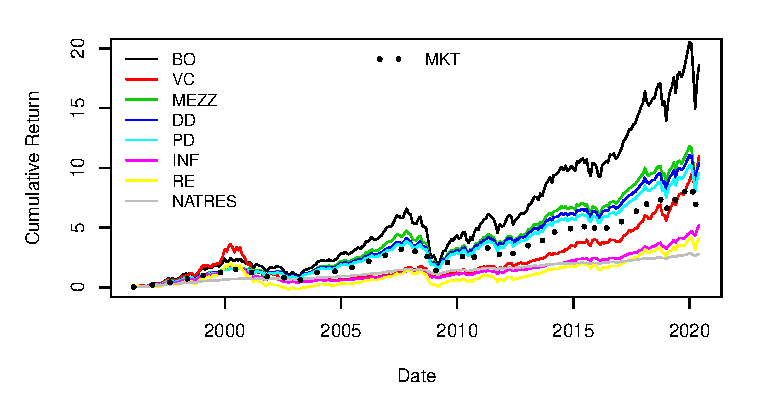
\includegraphics{Figures/Cumulative_Returns.eps}
%	\caption{PREQIN 2020:  Cumulative USD returns implied by the MSCI World factor models from Table 
% \ ref{tab:average_coefs} from 1996-01-31 until 2020-05-31.}
%%\end{figure}


\begin{figure}[H]
	\centering
	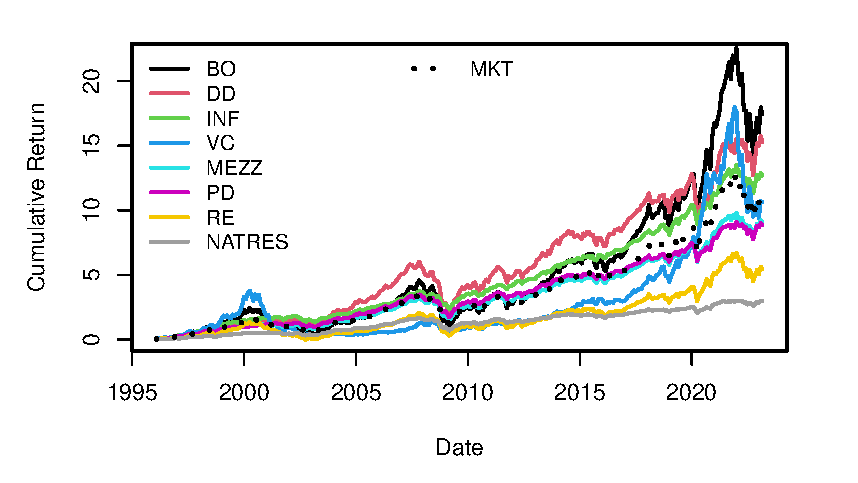
\includegraphics{Figures/Cumulative_Returns_2023_1996.eps}
	\caption{PITCHBOOK 2023: Cumulative USD returns implied by the five-factor models from Table \ref{tab:average_coefs_2023} from 1996-01-31 until 2023-02-28.}
	\label{fig:cum_returns_2023}   
\end{figure}




\subsection{Estimating idiosyncratic returns for BO funds}
\label{sec:idiosyncratic_BO}

In this section, we apply the idiosyncratic return estimation method described in subsection \ref{sec:error_term_estimation} for BO funds\footnote{We refrain from estimating the $e$ time series for other fund types because a full run takes about 100 hours on a 2023 MacBookPro with 12 CPU cores and parallel processing.}.
Here we use a starting point an ensemble of the MSCI market factors similar to the one described in Table \ref{tab:average_coefs_2023}.
Now we however only include fund-size-weighted datasets to reduce the long computation time that comes with this brute force approach.
Specifically, we use an ensemble of 40 two-factor models $4 \times 2 \times 5$  with (i) second factors (HML, SMB, HDY-MKT, QLT-MKT) (ii) quadratic and least absolute deviance loss function $L()$, and (iii) maximum months 120, 150, 180, 210, 240.
The average factor loadings of the five-factor model are fortunately very similar to the ones from Table \ref{tab:average_coefs_2023}:  
MKT-RF (1.46), 
HML (-0.09), 
SMB (-0.10), 
HDY-MKT (-0.15), and 
QLT-MKT (-0.09).

In the second step, we apply componetwise $L_2$ boosting (CLB) with 200 iterations for each two-factor ensemble, a damper factor of 0.33, and return bounds of plus and minus $100\%$.
For each of the 40 ensembles, we start with a vector of 307 zeros for $e$  (i.e. 307 monthly observations from 1996-12-31 until 2022-06-30).
After all CLB algorithms have been terminated, we average over all 40 error term series and public factor models to obtain our final estimate for $e$ and $\beta$.
Since only 46/307=15\% are filled with values other than zero in the final $e$ vector, our estimated error term series can be considered relatively sparse.
Yet three quarters exhibit quite extreme idiosyncratic returns of around +30\% or larger as depicted in Figure \ref{fig:clb_idio}.

\begin{figure}[H]
	\centering
	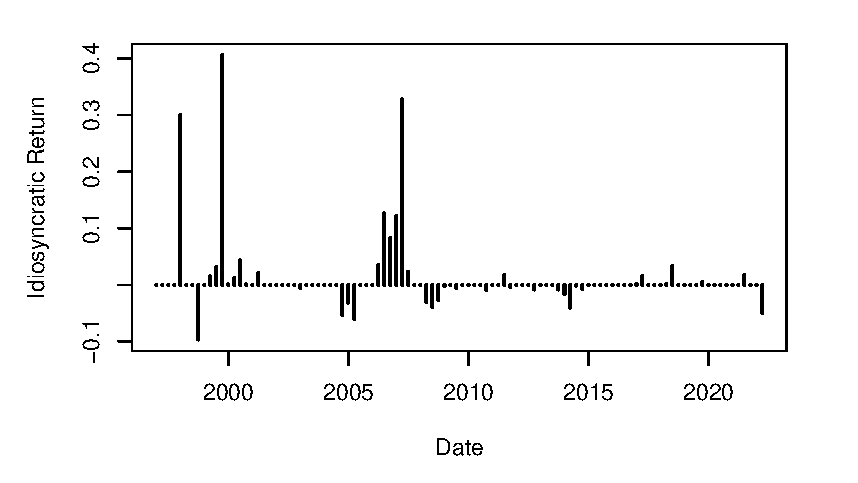
\includegraphics{Figures/ErrorSeriesBO}
	\caption{Idiosyncratic returns estimated by componentwise $L_2$ boosting for fund type BO in the period from 1996-12-31 until 2022-03-31.}
	\label{fig:clb_idio}
\end{figure}

For illustration and comparison with other BO return series, we map the monthly returns to quarterly returns in Figures \ref{fig:clb_idio} and \ref{fig:clb_total} and analyze the period from 1996-12-31 until 2022-03-31.
Figure \ref{fig:clb_total} nicely depicts that adding the error term estimates to our public factor model closely aligns the Public Factors + Error series to the NAV returns of Cambridge Associates (CA) and Pitchbook\footnote{Because of missing data, we fill the first quarters of the Pitchbook series with CA returns (from 1996-12-31 until 1999-09-30).}.
The Pearson correlation coefficients between our Public Factors + Error series and the CA and Pitchbook series are 78\% and 72\%, respectively.
The quarterly average return is relatively high in all three series with 4.5\% (Public Factors + Error), 3.8\% (CA), and 3.7\% (Pitchbook).
However, the standard deviation is considerably larger in our Public Factors + Error series with 15.3\% compared to 5.7\% and 5.1\% observed for CA and Pitchbook NAV returns, respectively.
For comparison, the MSCI Market [Public Factors] return exhibits a 2.7\% [3.4\%] average quarterly return with a standard deviation of 8.7\% [13.8\%].
Interestingly, the MSCI Market return and the public factor model return still exhibit a similar pattern in Figure \ref{fig:clb_total}.
Adding our sparse error term vector $e$ seems to visually transform a public return time series into a NAV return time series.
However the observed autocorrelation function values for lags 1 and 2 are considerably smaller in our Public Factors + Error series with 12.4\% and 12.0\% than in the CA (35.1\% and 30.4\%) and Pitchbook (40.6\% and 34.6\%) case.
Our boosting procedure thus can generate return proxies that do not suffer from the smoothing and staleness problems associated with NAV returns.

\begin{figure}[H]
	\centering
	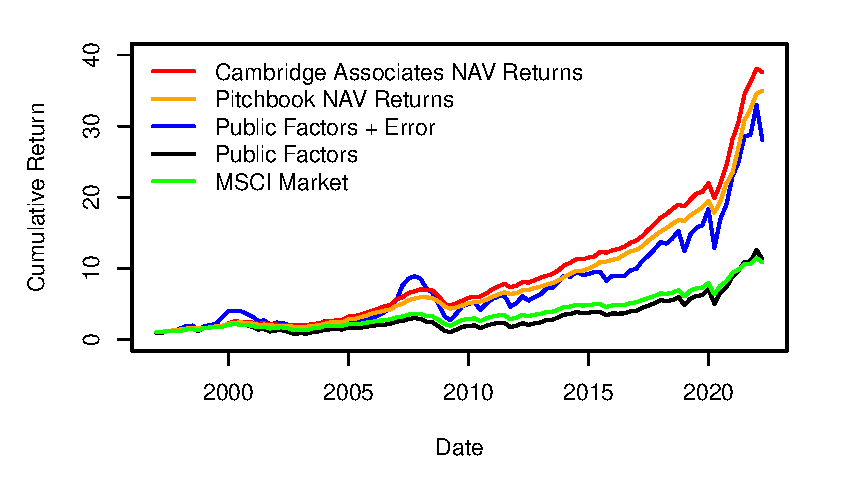
\includegraphics{Figures/TotalErrorSeriesBO}
	\caption{
		Comparison between the total returns for fund type BO implied by our two-factor ensemble and our two-factor ensemble plus the error term from Figure \ref{fig:clb_idio}.
		Both series are contrasted against the NAV Return indices provided by Cambridge Associates and Pitchbook and the MSCI stock market index in the period 1996-12-31 until 2022-03-31.
		}
	\label{fig:clb_total}
\end{figure}

\begin{figure}[H]
	\centering
	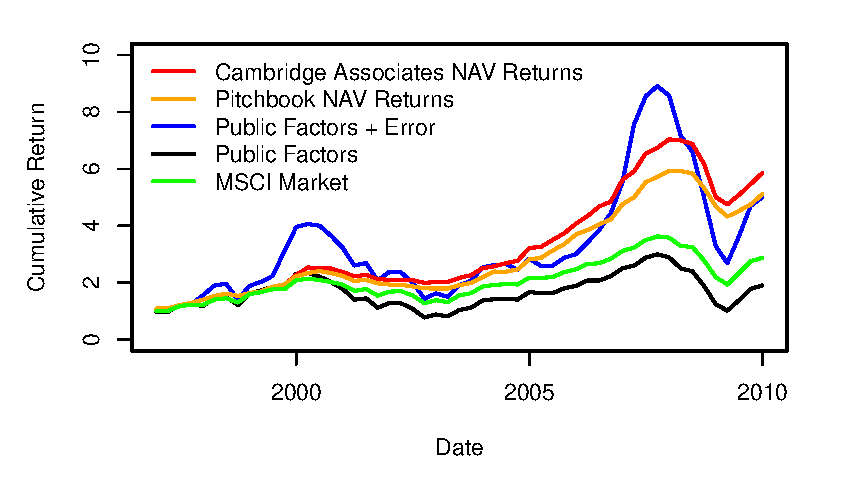
\includegraphics{Figures/TotalErrorSeriesBOpre2010}
	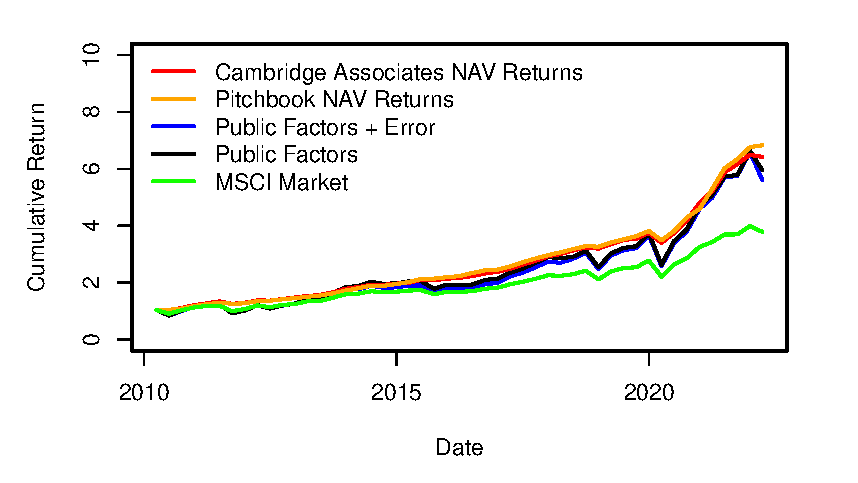
\includegraphics{Figures/TotalErrorSeriesBOpost2010}
	\caption{
		In these two subplots, we split the full time series from Figure \ref{fig:clb_total} into a pre-2010 and post-2010 period.
	}
	\label{fig:clb_pre_post_2010}
\end{figure}




In Figure \ref{fig:clb_pre_post_2010}, we split Figure \ref{fig:clb_total} in a pre-2010 and a post-2010 period.
We observe a big difference between the Average 2-Factor Models and the Average 2-Factor Models + Errors series in the period before 2010.
However after 2010, Public Factors and the Average 2-Factor Models return seem both closely aligned with the CA and Pitchbook NAV return indices.
Certainly, this result does not come by surprise as Figure \ref{fig:clb_idio} displays all large error terms before 2010.
From these analysis it remains unclear if the time-consuming error term estimation is always necessary since the average of the two-factor models alone can adequately price BO cash flows in the more recent past.


\subsection{Integrated public and private risk management}
\label{sec:integrated_risk}

In typical applications, we want to use our SDF models to analyze a blended portfolio of different private capital funds rather than investigate the factor exposure of a specific fund type.
In this case, we favor the bottom-up aggregation of SDF models to avoid overfitting.
Here, it is also straightforward to match the regional factor indices fund by fund.
In contrast, top-down selection of the 'best' SDF model for portfolio-level cash flows is likely to overfit with strongly varying SDF models for a given portfolio over time.

We consider two sets of ensembles when determining the factor exposure of actual PE portfolios.
The balanced ensemble is the set of all valid models for a given fund type, i.e., exactly the set $M^*$ as defined in subsection \ref{sec:model_averaging}.
The best ensemble is the size-$M^{**}$ subset of the balanced ensemble containing SDFs that best describes a given fund's cash flows in terms of absolute net present value error. 
Consequently, the number of components in the best ensemble is smaller than in the balanced ensemble $M^{**} \leq M^*$.
The comparison of the best and balanced model coefficients assesses how much the benchmarked portfolio's investment style differs from the average factor exposure of similar private capital portfolios.

For a sample portfolio of 100 funds visualized in figure \ref{fig:coef_barchart_100_pofo}, we see that the balanced model exhibits a MKT-RF coefficient slightly larger than one but the best SDF model MKF-RF coefficient is closer to 1.2.
This result implies higher than average market exposure for our portfolio.
Similarly, the best factor coefficients for HDY-MKT, QLT-MKT, and SMB are also higher than for the balanced ensemble.
Only the HML factor coefficient is basically the same for the best and balanced model.

Assume the asset owner of this PE portfolio is also invested in public markets.
For an integrated risk management application, the factor model derived by the best ensemble can be used as a public factor representation of the PE portfolio.
Established factor representations of any (public or private) portfolio shall be easily compatible with the asset owner's risk management framework.
Relevant methods to calculate risk measures like volatility, value-at-risk, or expected shortfall for public factor models shall be readily available in any investment risk department. 
This general approach works best if (i) the PE portfolio is diversified, and (ii) the public portfolio is still considerably larger than the PE allocation.
These conditions render an SDF model tracking error that is small in (i) absolute and (ii) relative terms and can thus be neglected.

\begin{figure}[H]
	\centering
	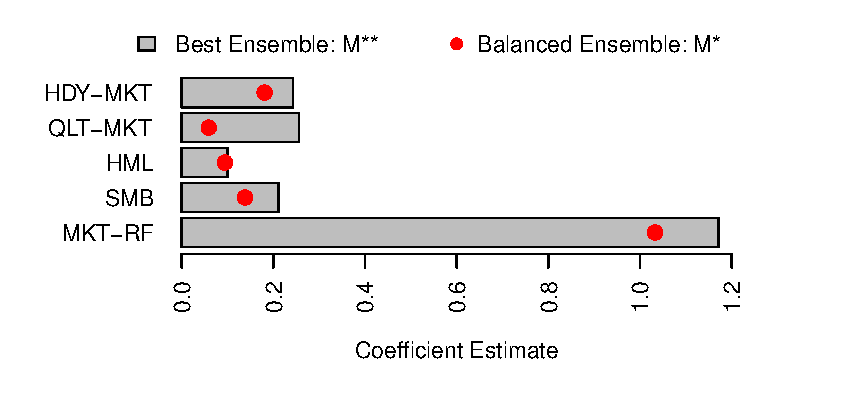
\includegraphics{Figures/Coefs100Pofo}
	\caption{Coefficient estimates of best and balanced linear SDF model for a sample portfolio consisting of 100 private capital funds.}
	\label{fig:coef_barchart_100_pofo}
\end{figure}



\section{Conclusion}
\label{sec:conclusion}

In this paper, we present a simple ensemble method to translate private equity cash flows into a public factor model and an error term time series. 
It can be used to (i) investigate public market factor exposures of private equity fund types (strategies) and to (ii) analyze actual private equity portfolios in order to enable the use of factor loadings in integrated risk management, establishing a common basis to compare the risk exposure of public and private asset portfolios. 
This novel type of analysis can complement more traditional methods of describing style and risk of private equity investments and yields additional insight for investors.
Our error term analysis shows for Buyout funds that before 2010 the error term played an important role in describing BO total returns; after 2010 the public factor model alone sufficed to price BO cash flows.
 
As a further perspective, we can amend our (i) simple ensemble approach for the public factor model and (ii) brute-force componentwise $L_2$ boosting for the error term by more efficient machine learning algorithms \citep{B12}.
Additionally, as already briefly mentioned in the article, we can apply cross-validation techniques to obtain the set of valid SDF models in a more reliable way than our simple quantile-based procedure.

%% References
\bibliographystyle{apalike}
\bibliography{ref}

% Appendix
\clearpage


\section{Pitchbook}
\label{sec:pitchbook}




\newcommand{\scaleWidth}{14cm}

% latex table generated in R 4.2.1 by xtable 1.8-4 package
% Thu May 11 10:54:20 2023
\begin{table}[ht]
	\centering
	\resizebox{\scaleWidth}{!}{% use resizebox with textwidth
		\begin{tabular}{lllllll}
			Type & MKT-RF & HML & SMB & HDY-MKT & QLT-MKT & Alpha \\ 
			\hline
			\hline
			%ALL & 1.23 (0.24) & -0.13 (0.06) & -0.18 (0.07) & -0.26 (0.13) & 0.04 (0.1) & -0.007 (0.02) \\ 
			BO & 1.33 (0.27) & -0.09 (0.04) & -0.14 (0.05) & -0.18 (0.09) & -0.11 (0.07) & 0.007 (0.017) \\ 
			DD & 0.83 (0.28) & 0.27 (0.06) & 0.35 (0.04) & 0.51 (0.08) & -0.4 (0.07) & 0.031 (0.043) \\ 
			%FOF & 0.56 (1.77) & -0.04 (0.25) & -0.51 (0.39) & -0.28 (0.79) & -0.27 (1.27) & 0.126 (0.245) \\ 
			INF & -0.29 (0.75) & -0.06 (0.11) & -0.31 (0.35) & -0.33 (0.43) & 0.46 (0.67) & 0.104 (0.1) \\ 
			MEZZ & 0.58 (0.17) & 0.03 (0.04) & 0.13 (0.05) & 0.06 (0.06) & -0.09 (0.09) & 0.024 (0.017) \\ 
			NATRES & 0.7 (0.35) & 0.06 (0.12) & 0.17 (0.18) & 0.17 (0.18) & -0.4 (0.33) & -0.019 (0.067) \\ 
			PD & 0.19 (0.43) & 0.15 (0.04) & 0.17 (0.05) & 0.24 (0.18) & -0.22 (0.23) & 0.068 (0.051) \\ 
			%PE & 1.32 (0.28) & -0.16 (0.08) & -0.19 (0.1) & -0.28 (0.17) & 0.11 (0.1) & -0.005 (0.023) \\ 
			RE & 2.02 (0.37) & 0.1 (0.08) & -0.07 (0.15) & 0.04 (0.19) & -0.55 (0.16) & -0.063 (0.047) \\ 
			%SEC & 1.63 (0.46) & -0.16 (0.05) & -0.15 (0.11) & -0.22 (0.16) & 0.32 (0.25) & -0.031 (0.036) \\ 
			VC & 1.41 (0.66) & -0.53 (0.08) & -0.7 (0.04) & -0.97 (0.18) & 0.63 (0.1) & -0.03 (0.071) \\ 
			\hline
			MKT & 1 & 0 & 0 & 0 & 0 & 0 \\ 
			\hline
			\hline
		\end{tabular}
	}
	\caption{
		PITCHBOOK 2023 ALPHA: Multivariate five-factor models obtained by simple coefficient averaging (with standard deviations in parenthesis).
		The ``Alpha'' term gives the average monthly outperformance.
	} 
	\label{tab:average_coefs_2023_alpha}
\end{table}


% latex table generated in R 4.2.1 by xtable 1.8-4 package
% Wed Jun 28 10:08:33 2023
\begin{table}[ht]
	\centering
	\begin{tabular}{llllll}
		Type & MKT & TERM & CORP & HY & LIQ \\ 
		\hline
		\hline
		ALL & 1.49 (0.14) & -0.25 (0.09) & -1.08 (0.34) & -0.62 (0.22) & -0.18 (0.05) \\ 
		BO & 1.56 (0.11) & -0.15 (0.01) & -0.75 (0.1) & -0.4 (0.02) & -0.01 (0.07) \\ 
		DD & 0.52 (0.12) & 0.34 (0.07) & 1.39 (0.17) & 0.73 (0.15) & 0.37 (0.06) \\ 
		FOF & 1.45 (0.21) & -0.3 (0.08) & -1.34 (0.22) & -0.9 (0.34) & -0.37 (0.17) \\ 
		INF & 0.59 (0.15) & 0.21 (0.07) & 0.62 (0.32) & 0.63 (0.16) & 0.24 (0.09) \\ 
		MEZZ & 0.6 (0.1) & 0.25 (0.08) & 0.78 (0.39) & 0.41 (0.17) & 0.23 (0.06) \\ 
		NATRES & 0.37 (0.11) & -0.23 (0.19) & 0.16 (0.42) & -0.42 (0.44) & 0.17 (0.18) \\ 
		PD & 0.4 (0.24) & 0.39 (0.23) & 1.24 (0.29) & 0.81 (0.34) & 0.23 (0.12) \\ 
		PE & 1.62 (0.13) & -0.23 (0.1) & -0.99 (0.37) & -0.58 (0.25) & -0.17 (0.09) \\ 
		RE & 1.47 (0.33) & -0.58 (0.17) & -3.44 (0.23) & -1.93 (0.41) & -0.49 (0.1) \\ 
		SEC & 1.71 (0.19) & -0.23 (0.1) & -0.97 (0.61) & -0.87 (0.44) & -0.25 (0.15) \\ 
		VC & 2.4 (0.42) & -0.75 (0.11) & -3.77 (0.79) & -2.21 (0.36) & -0.57 (0.05) \\ 
		\hline
		MKT & 1 & 0 & 0 & 0 & 0 \\ 
		\hline
		\hline
	\end{tabular}
	\caption{PITCHBOOK IBOXX MIX 2023: 
		Average coefficients of iBoxx factor models with standard deviation in parentheses.} 
	\label{tab:average_coefs_iboxx}
\end{table}


\iffalse

% latex table generated in R 4.2.1 by xtable 1.8-4 package
% Wed Jun 28 10:44:39 2023
\begin{table}[ht]
	\centering
	\begin{tabular}{rrrrrr}
		& Mean & Stdv & Mean.ex & Stdv.ex & Sharpe \\ 
		\hline
		\hline
		ALL & 0.107 & 0.239 & 0.091 & 0.219 & 0.414 \\ 
		BO & 0.123 & 0.256 & 0.107 & 0.236 & 0.453 \\ 
		DD & 0.083 & 0.131 & 0.067 & 0.109 & 0.613 \\ 
		FOF & 0.094 & 0.229 & 0.078 & 0.209 & 0.372 \\ 
		INF & 0.076 & 0.129 & 0.060 & 0.107 & 0.565 \\ 
		MEZZ & 0.078 & 0.132 & 0.062 & 0.110 & 0.568 \\ 
		NATRES & 0.041 & 0.082 & 0.026 & 0.057 & 0.452 \\ 
		PD & 0.070 & 0.111 & 0.054 & 0.088 & 0.614 \\ 
		PE & 0.119 & 0.260 & 0.102 & 0.241 & 0.425 \\ 
		RE & 0.070 & 0.218 & 0.054 & 0.199 & 0.271 \\ 
		SEC & 0.122 & 0.273 & 0.106 & 0.254 & 0.418 \\ 
		VC & 0.133 & 0.354 & 0.116 & 0.336 & 0.345 \\ 
		\hline
		MKT & 0.089 & 0.177 & 0.073 & 0.156 & 0.469 \\ 
		\hline
		\hline
	\end{tabular}
	\caption{
		PITCHBOOK IBOXX MIX 2023:
		Annualized returns of iBoxx five-factor models.
		The underlying monthly returns are based on iBoxx bond indices (for TERM, CORP, HY, LIQ) and the MSCI World for the MKT factor (in USD) from 1999-01-31 to 2023-02-28.
	} 
	\label{tab:ann_returns_iboxx}
\end{table}
\fi

\clearpage


\begin{figure}[H]
	\centering
	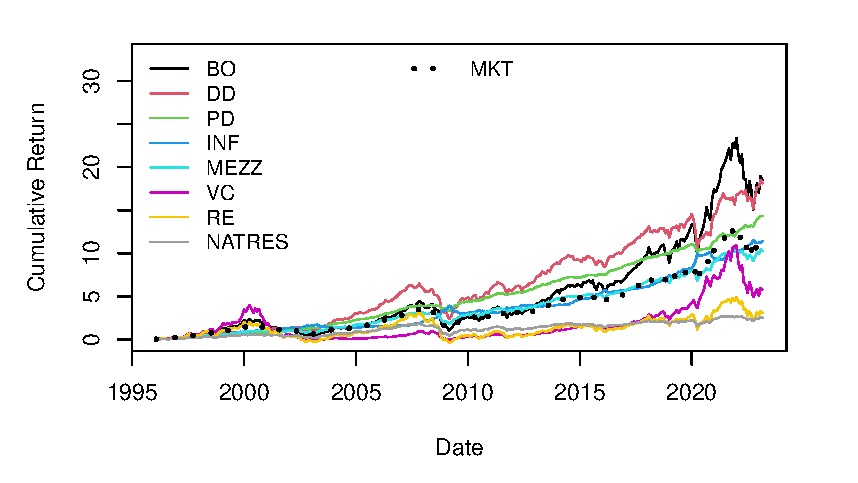
\includegraphics{Figures/Cumulative_Returns_2023_Alpha.eps}
	\caption{PITCHBOOK 2023 ALPHA: Cumulative USD returns implied by the MSCI World factor models from Table \ref{tab:average_coefs_2023} from 1999-01-31 until 2023-02-28.}
	\label{fig:cum_returns_2023_alpha}   
\end{figure}


\begin{figure}[H]
	\centering
	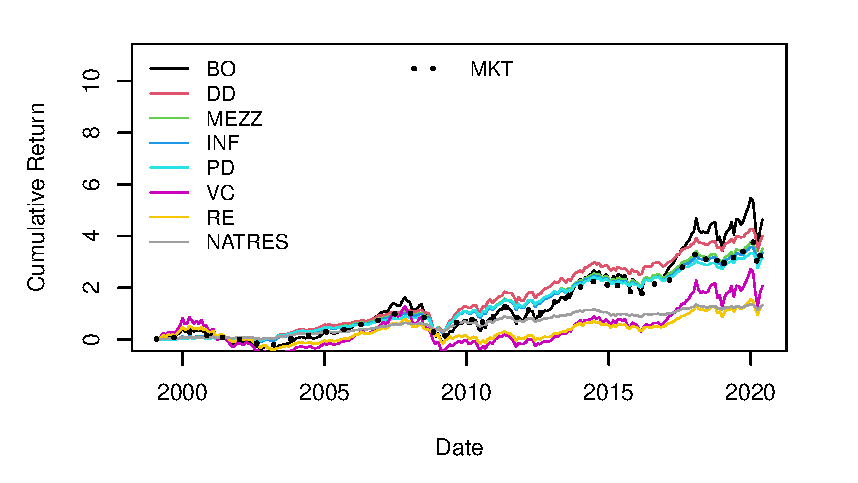
\includegraphics{Figures/Cumulative_Returns_2023_Bond.eps}
	\caption{PITCHBOOK 2023 BOND: Cumulative USD returns implied by the MSCI World factor models from Table \ref{tab:average_coefs_2023} from 1999-01-31 until 2023-02-28.}
	\label{fig:cum_returns_2023_iboxxx}
\end{figure}


\clearpage


\section{Preqin}
\label{sec:preqin}


% latex table generated in R 3.4.2 by xtable 1.8-4 package
% Wed Jul  1 13:54:55 2020
\begin{table}[ht]
	\centering
	\begin{tabular}{l@{\hskip 0.3in}l@{\hskip 0.2in}l@{\hskip 0.2in}l@{\hskip 0.2in}l@{\hskip 0.2in}l@{\hskip 0.1in}}
		Type & MKT-RF & HML & SMB & HDY-MKT & QLT-MKT \\ 
		\hline
		\hline
		BO & 1.33 (0.15) & -0.15 (0.12) & 0.2 (0.03) & 0.3 (0.1) & 0.21 (0.05) \\ 
		DD & 0.96 (0.09) & -0.11 (0.04) & 0.21 (0.01) & 0.14 (0.1) & 0.16 (0.05) \\ 
		%FOF & 1.22 (0.23) & -0.43 (0.09) & -0.24 (0.05) & -0.54 (0.09) & -0.01 (0.04) \\ 
		INF & 0.71 (0.22) & -0.37 (0.06) & -0.33 (0.13) & -0.47 (0.35) & 0.36 (0.11) \\ 
		MEZZ & 1.08 (0.13) & 0.06 (0.1) & 0.14 (0.04) & 0.16 (0.1) & 0.06 (0.11) \\ 
		NATRES & 0.36 (0.27) & -0.04 (0.22) & -0.02 (0.22) & 0.16 (0.36) & 0.11 (0.17) \\ 
		PD & 0.96 (0.08) & -0.07 (0.04) & 0.16 (0.03) & 0.06 (0.09) & 0.15 (0.04) \\ 
		%PE & 1.35 (0.16) & -0.2 (0.09) & 0.14 (0.07) & 0.24 (0.12) & 0.17 (0.04) \\ 
		RE & 1.14 (0.44) & -0.3 (0.16) & -0.42 (0.13) & -0.91 (0.15) & -0.4 (0.1) \\ 
		%SEC & 1.34 (0.25) & -0.36 (0.17) & -0.2 (0.07) & -0.29 (0.33) & 0.13 (0.04) \\ 
		VC & 1.02 (0.67) & -0.61 (0.11) & -0.42 (0.03) & -0.75 (0.14) & 0.84 (0.61) \\ 
		\hline
		MKT & 1 & 0 & 0 & 0 & 0 \\ 
		\hline
		\hline
	\end{tabular}
	\caption{
		PREQIN 2020: Multivariate five-factor models obtained by simple coefficient averaging (with standard deviations in parenthesis).
	} 
	\label{tab:average_coefs_preqin_2020}
\end{table}


% latex table generated in R 3.4.2 by xtable 1.8-4 package
% Fri Jul  3 14:50:53 2020
\begin{table}[ht]
	\centering
	\begin{tabular}{lrrrrr}
		Type & \multicolumn{4}{c}{Annualized Return} & Sharpe Ratio \\ 
		\cmidrule(r){2-5}
		& mean.R & stdv.R & mean.R-RF & stdv.R-RF & mean/stdv.R-RF \\ 
		\hline
		\hline
		BO & \textbf{0.152} & 0.195 & \textbf{0.125} & 0.196 & 0.641 \\ 
		DD & 0.116 & 0.144 & 0.091 & 0.144 & 0.630 \\ 
		%FOF & 0.120 & 0.200 & 0.094 & 0.200 & 0.470 \\ 
		INF & 0.085 & 0.119 & 0.060 & 0.119 & 0.506 \\ 
		MEZZ & 0.120 & 0.162 & 0.094 & 0.162 & 0.581 \\ 
		NATRES & 0.057 & \textbf{0.049} & 0.033 & \textbf{0.049} & \textbf{0.671} \\ 
		PD & 0.113 & 0.143 & 0.087 & 0.143 & 0.610 \\ 
		%PE & 0.151 & 0.200 & 0.125 & 0.200 & 0.624 \\ 
		RE & 0.092 & 0.203 & 0.067 & 0.203 & 0.329 \\ 
		%SEC & 0.137 & 0.207 & 0.111 & 0.207 & 0.537 \\ 
		VC & 0.124 & 0.176 & 0.099 & 0.176 & 0.561 \\ 
		\hline
		MKT & 0.107 & 0.152 & 0.082 & 0.152 & 0.536 \\ 
		\hline
		\hline
	\end{tabular}
	\caption{
		PREQIN 2020: 
		Annualized average returns, standard deviations (annualized by the square root of time formula), and Sharpe ratios (i.e., the ratio of mean.R-RF to stdv.R-RF) implied by the five-factor models from table \ref{tab:average_coefs_preqin_2020}. 
		The underlying monthly returns are based on MSCI World style indices (in USD) from 1996-01-31 to 2020-05-31.
	} 
	\label{tab:ann_returns_preqin_2020}
\end{table}


\begin{figure}[H]
	\centering
	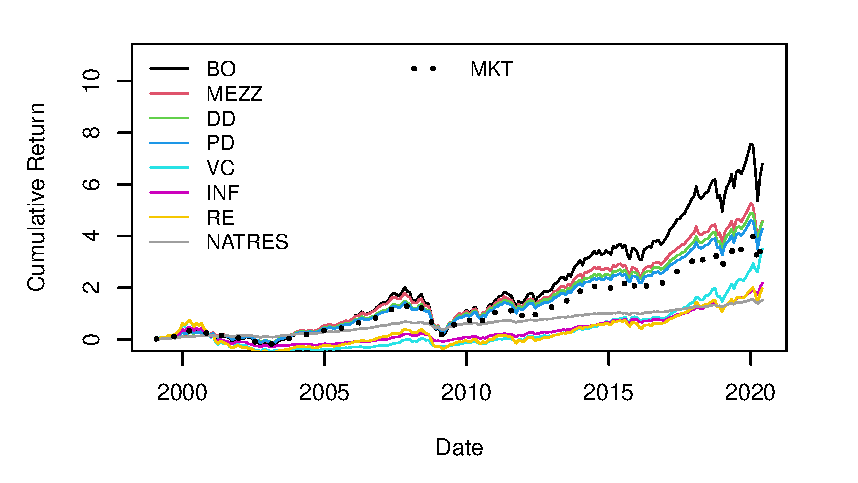
\includegraphics{Figures/Cumulative_Returns_2020.eps}
	\caption{
		PREQIN 2023: Cumulative USD returns implied by the MSCI World factor models from Table \ref{tab:average_coefs_preqin_2020} from 1999-01-31 until 2023-02-28.}
	\label{fig:cum_returns_preqin}   
\end{figure}



% latex table generated in R 3.6.1 by xtable 1.8-4 package
% Tue Jul 28 12:13:36 2020
\begin{table}[ht]
	\centering
	\begin{tabular}{lrrrrrrrr}
		Vintage & BO & DD & INF & MEZZ & NATRES & PD & RE & VC \\ 
		\hline
		\hline
		%1983 &   0 &   0 &   0 &   0 &   0 &   0 &   0 &   0 \\ 
		1984 &   0 &   0 &   0 &   0 &   0 &   0 &   0 &   1 \\ 
		1985 &   3 &   0 &   0 &   0 &   0 &   0 &   0 &   4 \\ 
		1986 &   2 &   0 &   0 &   1 &   0 &   1 &   0 &   4 \\ 
		1987 &   4 &   0 &   0 &   1 &   0 &   1 &   0 &   3 \\ 
		1988 &   7 &   0 &   0 &   0 &   0 &   0 &   0 &   2 \\ 
		1989 &   2 &   0 &   0 &   0 &   1 &   0 &   0 &   2 \\ 
		1990 &   5 &   1 &   0 &   0 &   0 &   1 &   0 &   6 \\ 
		1991 &   3 &   2 &   0 &   0 &   0 &   2 &   0 &   4 \\ 
		1992 &   9 &   2 &   0 &   2 &   1 &   4 &   1 &   7 \\ 
		1993 &   7 &   0 &   0 &   0 &   0 &   0 &   0 &   4 \\ 
		1994 &   9 &   1 &   0 &   2 &   1 &   3 &   1 &   7 \\ 
		1995 &  17 &   0 &   0 &   1 &   1 &   1 &   1 &  10 \\ 
		1996 &  16 &   2 &   0 &   2 &   0 &   4 &   4 &  10 \\ 
		1997 &  16 &   2 &   0 &   0 &   1 &   2 &   6 &  14 \\ 
		1998 &  30 &   1 &   0 &   3 &   2 &   4 &   3 &  23 \\ 
		1999 &  28 &   1 &   0 &   7 &   1 &   8 &   2 &  37 \\ 
		2000 &  32 &   3 &   0 &   4 &   0 &   7 &   6 &  67 \\ 
		2001 &  18 &   2 &   0 &   3 &   1 &   5 &   2 &  40 \\ 
		2002 &  24 &   4 &   1 &   2 &   2 &   6 &   2 &  24 \\ 
		2003 &  18 &   3 &   1 &   2 &   1 &   5 &   6 &  19 \\ 
		2004 &  29 &   2 &   4 &   3 &   2 &   5 &  10 &  29 \\ 
		2005 &  63 &   6 &   0 &   7 &   4 &  14 &  19 &  34 \\ 
		2006 &  76 &  10 &   5 &   5 &   3 &  16 &  34 &  41 \\ 
		2007 &  88 &  13 &   5 &   3 &   7 &  16 &  36 &  53 \\ 
		2008 &  76 &  12 &   3 &   6 &   8 &  21 &  35 &  40 \\ 
		2009 &  35 &   7 &   5 &   4 &   4 &  12 &  14 &  20 \\ 
		2010 &  53 &   9 &   9 &   7 &   8 &  18 &  40 &  21 \\ 
		2011 &  72 &   8 &  11 &   6 &   9 &  16 &  51 &  27 \\ 
		2012 &  69 &  14 &   4 &  11 &  11 &  26 &  42 &  25 \\ 
		2013 &  80 &  15 &  12 &   4 &   8 &  32 &  61 &  30 \\ 
		2014 &  88 &  13 &  12 &   5 &  15 &  31 &  56 &  36 \\ 
		2015 &  99 &  18 &  13 &   7 &   9 &  38 &  86 &  47 \\ 
		2016 & 108 &   8 &  16 &   8 &  16 &  29 &  63 &  56 \\ 
		2017 &  83 &  15 &  20 &   8 &  13 &  48 &  78 &  56 \\ 
		2018 &  88 &  22 &  18 &  11 &   8 &  54 &  71 &  55 \\ 
		2019 &  21 &   3 &   5 &   2 &   1 &  11 &  12 &  11 \\ 
		\hline
		Total & 1378 & 199 & 144 & 127 & 138 & 441 & 742 & 869 \\ 
		\hline
		\hline
	\end{tabular}
	\caption{PREQIN 2020: Number of funds per vintage year in the Preqin dataset used for estimation (Preqin cash flow data set as of 26th February 2020).} 
	\label{tab:preqin_data}
\end{table}


\newpage


% Factor Model Returns + Errors
\renewcommand{\segment}{PE}

\subsection{Preqin: Idiosyncratic returns for \segment \ funds}
\label{sec:preqin_errors_\segment}

\begin{figure}[H]
	\centering
	\includegraphics{Figures/q_factors/XErrorSeries\segment Preqin}
	\caption{Idiosyncratic returns estimated by componentwise $L_2$ boosting for fund type \segment \ in the period from 1990-03-31 until 2019-09-30.}
	\label{fig:preqin_clb_idio_\segment}
\end{figure}

\begin{figure}[H]
	\centering
	\includegraphics{Figures/q_factors/XTotalErrorSeries\segment Preqin}
	\caption{
		Comparison between the total returns for fund type \segment \ implied by our two-factor ensemble and our two-factor ensemble plus the error term from Figure \ref{fig:preqin_clb_idio_\segment}.
		Both series are contrasted against the NAV Return indices provided by Cambridge Associates and Pitchbook and the MSCI stock market index in the period 1990-03-31 until 2019-09-30.
	}
	\label{fig:preqin_clb_total_\segment}
\end{figure}

\begin{figure}[H]
	\centering
	\includegraphics{Figures/q_factors/XTotalErrorSeries\segment Preqinpre2010}
	\includegraphics{Figures/q_factors/XTotalErrorSeries\segment Preqinpost2010}
	\caption{
		In these two subplots, we split the full \segment \ time series from Figure \ref{fig:preqin_clb_total_\segment} into a pre-2010 and post-2010 period.
	}
	\label{fig:preqin_clb_pre_post_2010_\segment}
\end{figure}


% Factor Model Returns + Errors
\renewcommand{\segment}{VC}

\subsection{Preqin: Idiosyncratic returns for \segment \ funds}
\label{sec:preqin_errors_\segment}

\begin{figure}[H]
	\centering
	\includegraphics{Figures/q_factors/XErrorSeries\segment Preqin}
	\caption{Idiosyncratic returns estimated by componentwise $L_2$ boosting for fund type \segment \ in the period from 1990-03-31 until 2019-09-30.}
	\label{fig:preqin_clb_idio_\segment}
\end{figure}

\begin{figure}[H]
	\centering
	\includegraphics{Figures/q_factors/XTotalErrorSeries\segment Preqin}
	\caption{
		Comparison between the total returns for fund type \segment \ implied by our two-factor ensemble and our two-factor ensemble plus the error term from Figure \ref{fig:preqin_clb_idio_\segment}.
		Both series are contrasted against the NAV Return indices provided by Cambridge Associates and Pitchbook and the MSCI stock market index in the period 1990-03-31 until 2019-09-30.
	}
	\label{fig:preqin_clb_total_\segment}
\end{figure}

\begin{figure}[H]
	\centering
	\includegraphics{Figures/q_factors/XTotalErrorSeries\segment Preqinpre2010}
	\includegraphics{Figures/q_factors/XTotalErrorSeries\segment Preqinpost2010}
	\caption{
		In these two subplots, we split the full \segment \ time series from Figure \ref{fig:preqin_clb_total_\segment} into a pre-2010 and post-2010 period.
	}
	\label{fig:preqin_clb_pre_post_2010_\segment}
\end{figure}



% Factor Model Returns + Errors
\renewcommand{\segment}{RE}

\subsection{Preqin: Idiosyncratic returns for \segment \ funds}
\label{sec:preqin_errors_\segment}

\begin{figure}[H]
	\centering
	\includegraphics{Figures/q_factors/XErrorSeries\segment Preqin}
	\caption{Idiosyncratic returns estimated by componentwise $L_2$ boosting for fund type \segment \ in the period from 1992-06-30 until 2019-09-30.}
	\label{fig:preqin_clb_idio_\segment}
\end{figure}

\begin{figure}[H]
	\centering
	\includegraphics{Figures/q_factors/XTotalErrorSeries\segment Preqin}
	\caption{
		Comparison between the total returns for fund type \segment \ implied by our two-factor ensemble and our two-factor ensemble plus the error term from Figure \ref{fig:preqin_clb_idio_\segment}.
		Both series are contrasted against the NAV Return indices provided by Cambridge Associates and Pitchbook and the MSCI stock market index in the period 1990-03-31 until 2019-09-30.
	}
	\label{fig:preqin_clb_total_\segment}
\end{figure}

\begin{figure}[H]
	\centering
	\includegraphics{Figures/q_factors/XTotalErrorSeries\segment Preqinpre2010}
	\includegraphics{Figures/q_factors/XTotalErrorSeries\segment Preqinpost2010}
	\caption{
		In these two subplots, we split the full \segment \ time series from Figure \ref{fig:preqin_clb_total_\segment} into a pre-2010 and post-2010 period.
	}
	\label{fig:preqin_clb_pre_post_2010_\segment}
\end{figure}



\end{document}
